\documentclass{article}

% Language setting
% Replace `english' with e.g. `spanish' to change the document language
\usepackage[polish]{babel}
\usepackage[T1]{fontenc}

% Set page size and margins
% Replace `letterpaper' with`a4paper' for UK/EU standard size
\usepackage[letterpaper,top=2cm,bottom=2cm,left=3cm,right=3cm,marginparwidth=1.75cm]{geometry}

% Useful packages
\usepackage{amsmath}
\usepackage{graphicx}
\usepackage{setspace}
\usepackage{float}

\title{Aproksymacja interpolacyjna}
\author{Marcel Grużewski 193589}

\begin{document}
\maketitle

\singlespacing
\section{Wstęp}

\subsection{Cel projektu}
Celem projektu jest przeprowadzenie analizy metod interpolacji na przykładach tras wysokościowych.
Analizowane metody interpolacji to \textbf{metoda wykorzystująca wielomian interpolacyjny Lagrange’a},
oraz \textbf{metoda wykorzystująca funkcje sklejane trzeciego stopnia.}


\subsection{Czym jest interpolacja?}

Interpolacja to proces, który polega na znalezieniu wartości funkcji w punkcie, który nie jest bezpośrednio dostępny, ale może zostać oszacowany na podstawie wartości tej funkcji w innych punktach.

\subsection{Interpolacja Lagrange'a}

Interpolacja Lagrange'a to metoda interpolacji wielomianowej, która pozwala na znalezienie wielomianu interpolacyjnego bezpośrednio. Dla danej funkcji i zestawu punktów, metoda ta generuje wielomian, który przeszczepia się przez wszystkie te punkty. Formuła interpolacji Lagrange'a wyraża się jako:

\begin{align}
f(x) = \sum_{j=0}^{n} y_j L_j(x)
\end{align}

gdzie:

\begin{itemize}
    \item \( f(x) \) to wartość funkcji interpolowanej dla dowolnego argumentu \( x \),
    \item \( y_j \) to wartość funkcji w \( j \)-tym węźle,
    \item \( L_j(x) \) to \( j \)-ty element wielomianu Lagrange'a,
    \item \( x_j \) oznacza położenie znanych węzłów.
\end{itemize}

Elementy wielomianu Lagrange'a \( L_j(x) \) obliczamy według wzoru:

\begin{equation}
L_j(x) = \prod_{k=0, k \neq j}^{n} \frac{x - x_k}{x_j - x_k}
\end{equation}

\subsection{Interpolacja funkcjami sklejonymi}

Interpolacja funkcjami sklejanymi to metoda interpolacji, która polega na zastosowaniu wielomianów niskiego stopnia (np. wielomianów trzeciego stopnia) do przybliżenia funkcji w danym przedziale. W przeciwieństwie do interpolacji Lagrange'a, która generuje jeden wielomian interpolacyjny dla całego przedziału, interpolacja funkcjami sklejanymi dzieli przedział na mniejsze segmenty i dla każdego segmentu tworzy osobny wielomian. Następnie te wielomiany są "sklejane" razem, tworząc gładką funkcję, która przechodzi przez wszystkie punkty interpolacji.

Formuła interpolacji funkcjami sklejanymi wygląda następująco:

\[
S(x) = 
\begin{cases} 
s_1(x) & \text{dla } a \leq x < c \\
s_2(x) & \text{dla } c \leq x < d \\
s_3(x) & \text{dla } d \leq x \leq b 
\end{cases}
\]

gdzie:
\begin{itemize}
    \item \( S(x) \) to funkcja sklejana,
    \item \( s_i(x) \) to \( i \)-ty segment wielomianu sklejanego,
    \item \( a, b \) to granice przedziału,
    \item \( c, d \) to punkty, w których segmenty są połączone.
\end{itemize}

Elementy wielomianów sklejanego \( s_i(x) \) obliczamy indywidualnie dla każdego segmentu, zazwyczaj jako trzeci stopień wielomianu, który spełnia warunki interpolacji w punktach węzłowych tego segmentu oraz warunki ciągłości pierwszych i drugich pochodnych w punktach połączenia segmentów.

\subsection{Efekt Rungego}

Efekt Rungego to zjawisko występujące podczas interpolacji wielomianowej, szczególnie przy użyciu wielomianów wysokiego stopnia i równomiernie rozmieszczonych węzłów. Polega ono na tym, że funkcja interpolacyjna zaczyna oscylować i wykazuje duże błędy na krańcach przedziału interpolacji.

\begin{figure}[h]
    \centering
    \includegraphics[width=0.6\textwidth]{runge.png}
    \caption{Efekt Rungego}
\end{figure}

\subsection{Węzły Czebyszewa}

Węzły Czebyszewa to specjalne punkty używane w celu zminimalizowania błędów interpolacji wielomianowej i uniknięcia efektu Rungego. Zamiast używać równomiernie rozmieszczonych węzłów, węzły Czebyszewa są gęściej rozmieszczone na krańcach przedziału i rzadziej w jego środku. Są one zdefiniowane jako miejsca zerowe wielomianów Czebyszewa pierwszego rodzaju i dla n węzłów obliczane są z poniższego wzoru:

\begin{equation}
    x_i = \cos\left(\frac{{2i - 1} \pi}{2n}\right) \quad \text{dla} \quad i = 1, 2, \ldots, n
\end{equation}


Dzięki takiemu rozłożeniu węzłów, interpolacja wielomianowa staje się bardziej stabilna i dokładna, redukując oscylacje i błędy na krańcach przedziału. Węzły Czebyszewa są często wykorzystywane w praktyce do poprawy jakości interpolacji i uniknięcia problemów związanych z efektem Rungego.

\clearpage
\section{Wykorzystane dane}

W każdym zestawie danych jest 512 węzłów.

\subsection{Mount Everest}

\begin{figure}[h]
    \centering
    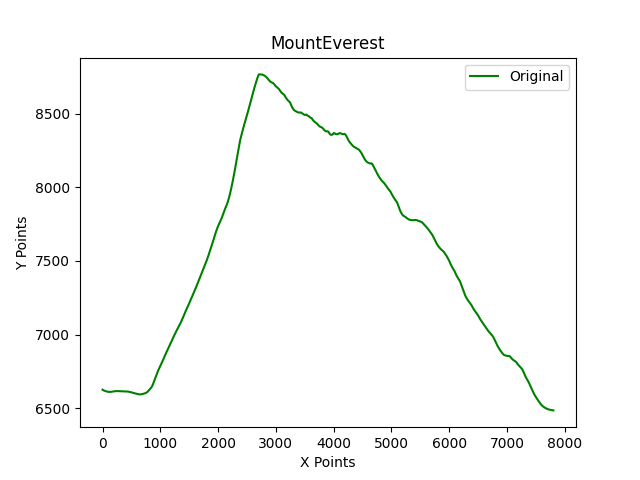
\includegraphics[width=0.6\textwidth]{plots/MountEverest_original.png}
    \caption{Mount Everest}
\end{figure}

\subsection{Spacerniak Gdańsk}

\begin{figure}[h]
    \centering
    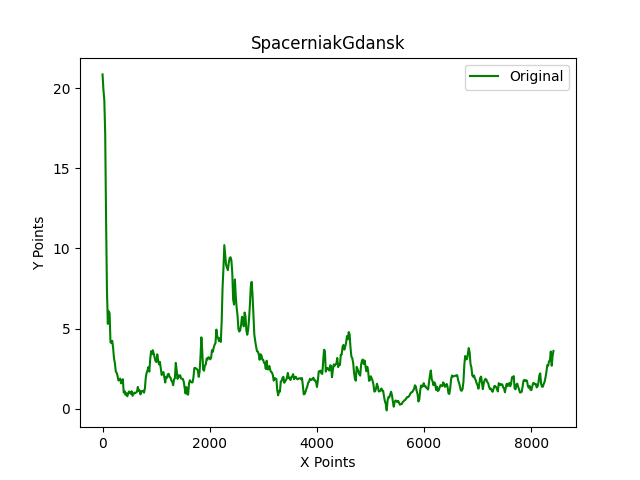
\includegraphics[width=0.6\textwidth]{plots/SpacerniakGdansk_original.png}
    \caption{Spacerniak Gdańsk}
\end{figure}

\subsection{Stałe}

\begin{figure}[H]
    \centering
    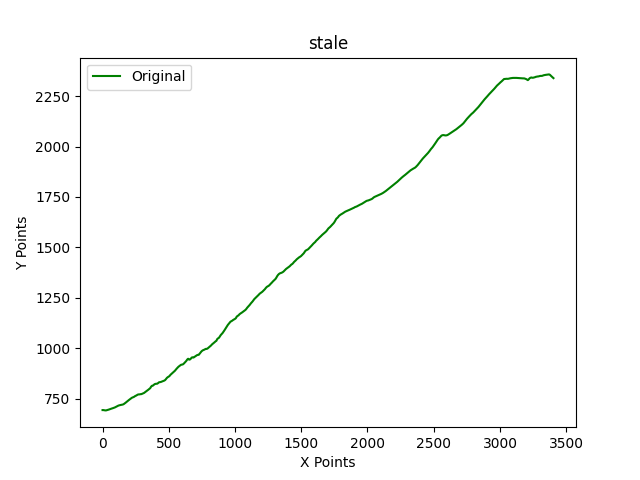
\includegraphics[width=0.6\textwidth]{plots/stale_original.png}
    \caption{Stałe}
\end{figure}

\subsection{Wielki Kanion Kolorado}

\begin{figure}[H]
    \centering
    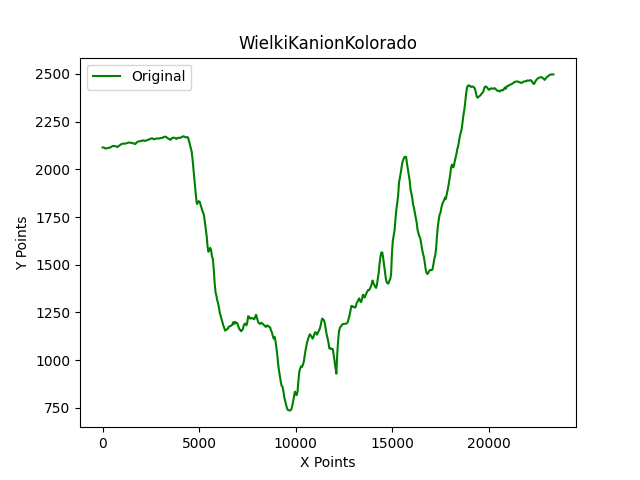
\includegraphics[width=0.6\textwidth]{plots/WielkiKanionKolorado_original.png}
    \caption{Wielki Kanion Kolorado}
\end{figure}

\clearpage
\section{Analiza podstawowa}

Analiza podstawowa będzie odbywać się na danych \textbf{Mount Everest} oraz \textbf{Spacerniak Gdańsk}. Będzie polegała na badaniu wpływu liczby punktów węzłowych na wyniki. Do przeprowadzenia analizy obu metod - \textbf{Lagrange'a} oraz \textbf{funkcji sklejonych trzeciego stopnia} wykorzystane zostana liczby węzłów \textbf{7, 14, 21, 28}.

\subsection{Spacerniak Gdańsk - interpolacja Lagrange'a}

\begin{figure}[H]
    \centering
    \begin{minipage}[b]{0.49\textwidth}
        \centering
        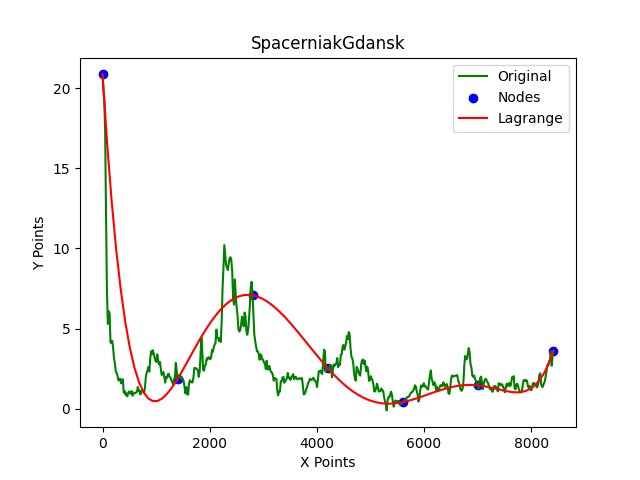
\includegraphics[width=\textwidth]{plots/SpacerniakGdansk_lagrange_7.png}
        \caption{7 węzłów}
        \label{fig:7nodes}
    \end{minipage}
    \hfill
    \begin{minipage}[b]{0.49\textwidth}
        \centering
        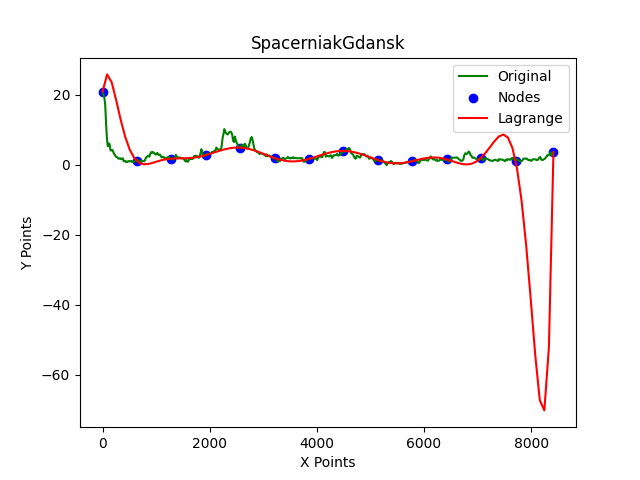
\includegraphics[width=\textwidth]{plots/SpacerniakGdansk_lagrange_14.png}
        \caption{14 węzłów}
        \label{fig:14nodes}
    \end{minipage}
\end{figure}
\begin{figure}[H]
    \centering
    \begin{minipage}[b]{0.49\textwidth}
        \centering
        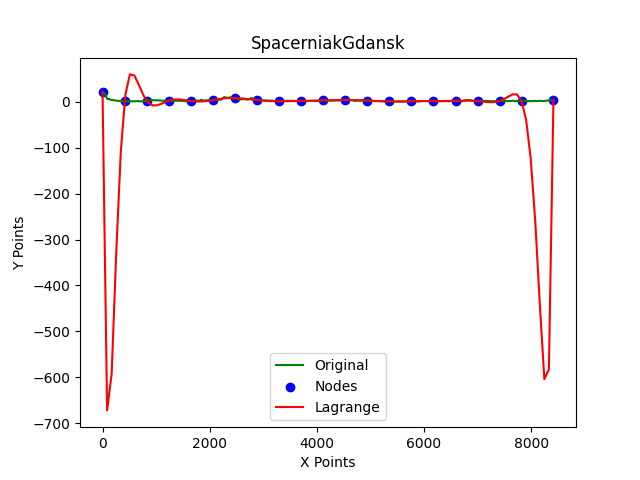
\includegraphics[width=\textwidth]{plots/SpacerniakGdansk_lagrange_21.png}
        \caption{21 węzłów}
        \label{fig:21nodes}
    \end{minipage}
    \hfill
    \begin{minipage}[b]{0.49\textwidth}
        \centering
        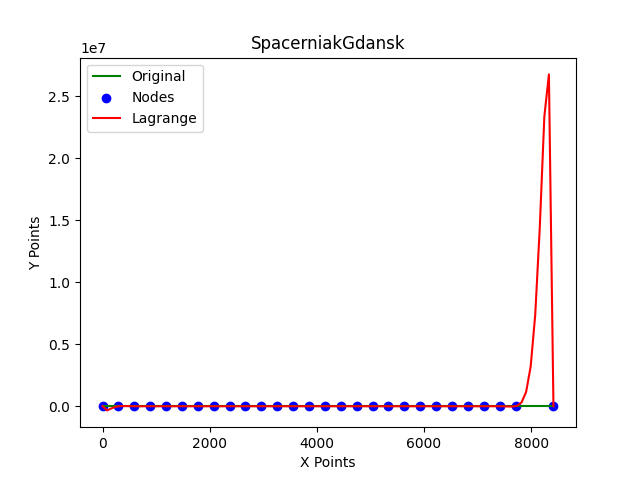
\includegraphics[width=\textwidth]{plots/SpacerniakGdansk_lagrange_28.png}
        \caption{28 węzłów}
        \label{fig:28nodes}
    \end{minipage}
\end{figure}

Jak widać przy użyciu równomiernie rozłożonych węzłów przy metodzie interpolacji Lagrange'a nasz wykres bardzo szybko napotyka efekt Rungego, który już przy 14 węzłach zaczyna wypłaszczać wykres, a przy większych ilościach kompletnie wypacza wykres.

\subsection{Spacerniak Gdańsk - interpolacja metodą funckji sklejanych}

\begin{figure}[H]
    \centering
    \begin{minipage}[b]{0.49\textwidth}
        \centering
        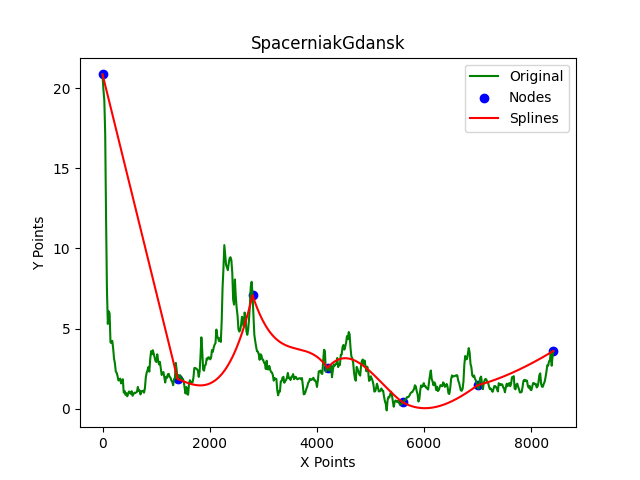
\includegraphics[width=\textwidth]{plots/SpacerniakGdansk_splines_7.png}
        \caption{7 węzłów}
        \label{fig:7nodes}
    \end{minipage}
    \hfill
    \begin{minipage}[b]{0.49\textwidth}
        \centering
        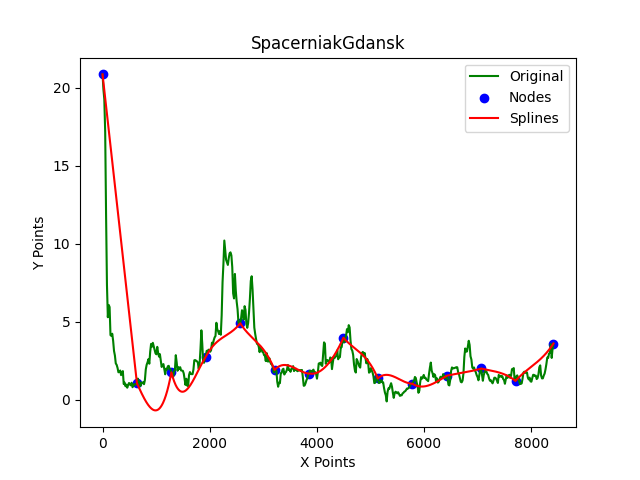
\includegraphics[width=\textwidth]{plots/SpacerniakGdansk_splines_14.png}
        \caption{14 węzłów}
        \label{fig:14nodes}
    \end{minipage}
\end{figure}
\begin{figure}[H]
    \centering
    \begin{minipage}[b]{0.49\textwidth}
        \centering
        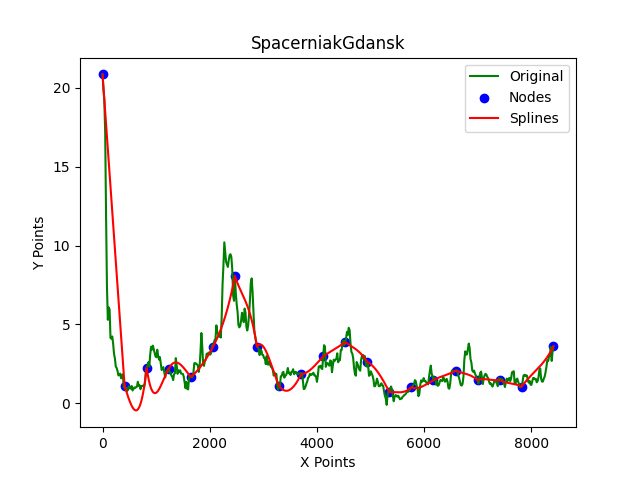
\includegraphics[width=\textwidth]{plots/SpacerniakGdansk_splines_21.png}
        \caption{21 węzłów}
        \label{fig:21nodes}
    \end{minipage}
    \hfill
    \begin{minipage}[b]{0.49\textwidth}
        \centering
        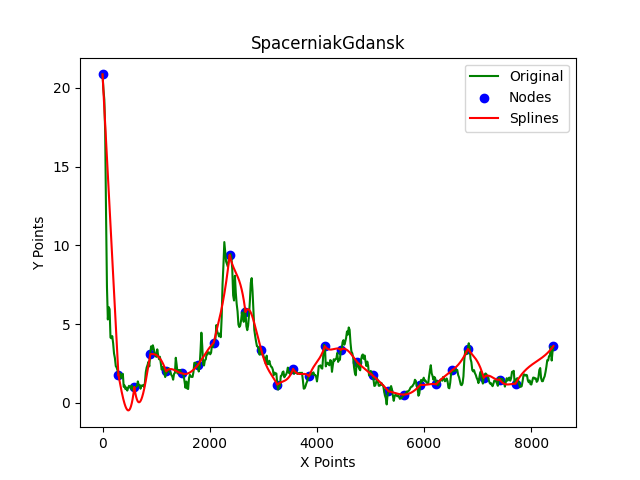
\includegraphics[width=\textwidth]{plots/SpacerniakGdansk_splines_28.png}
        \caption{28 węzłów}
        \label{fig:28nodes}
    \end{minipage}
\end{figure}

Dzięki tej metodzie jesteśmy w stanie uzyskać znacznie lepszy efekt, szczególnie porównując wykresy do tych z metody Lagrange'a. Tutaj już przy 21 węzłach jesteśmy zaobserwować zadowalającą dokładność.

\subsection{Mount Everest - interpolacja Lagrange'a}

\begin{figure}[H]
    \centering
    \begin{minipage}[b]{0.49\textwidth}
        \centering
        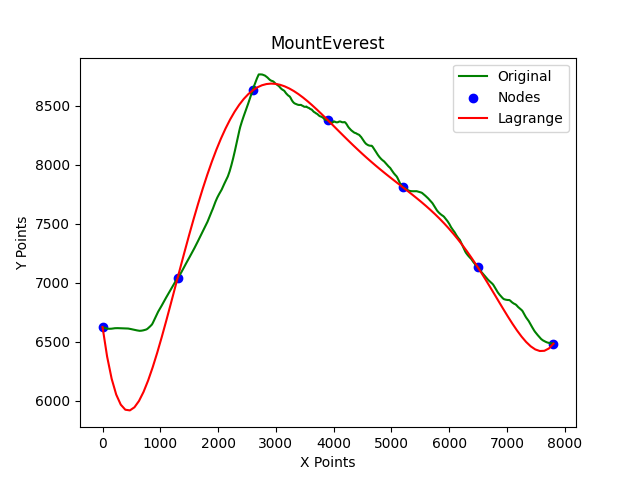
\includegraphics[width=\textwidth]{plots/MountEverest_lagrange_7.png}
        \caption{7 węzłów}
        \label{fig:7nodes}
    \end{minipage}
    \hfill
    \begin{minipage}[b]{0.49\textwidth}
        \centering
        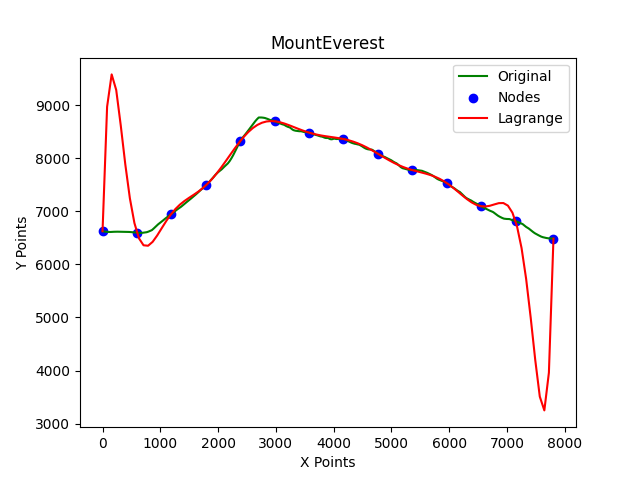
\includegraphics[width=\textwidth]{plots/MountEverest_lagrange_14.png}
        \caption{14 węzłów}
        \label{fig:14nodes}
    \end{minipage}
\end{figure}
\begin{figure}[H]
    \centering
    \begin{minipage}[b]{0.49\textwidth}
        \centering
        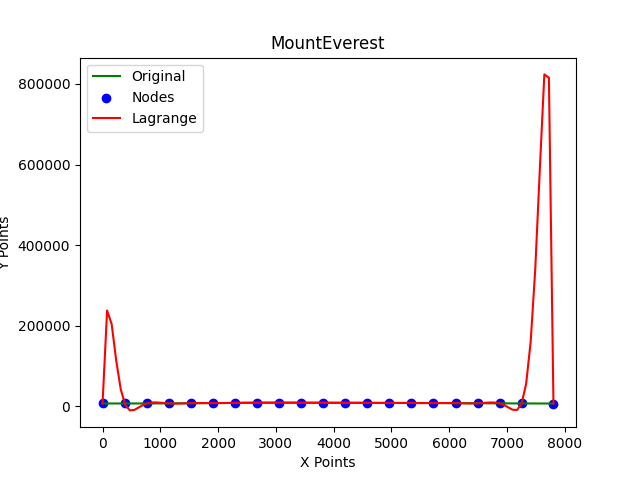
\includegraphics[width=\textwidth]{plots/MountEverest_lagrange_21.png}
        \caption{21 węzłów}
        \label{fig:21nodes}
    \end{minipage}
    \hfill
    \begin{minipage}[b]{0.49\textwidth}
        \centering
        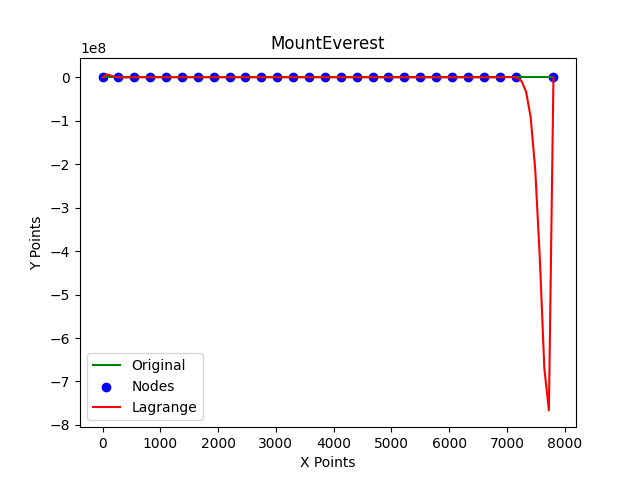
\includegraphics[width=\textwidth]{plots/MountEverest_lagrange_28.png}
        \caption{28 węzłów}
        \label{fig:28nodes}
    \end{minipage}
\end{figure}

Dla danych Mount Everest znowu widać duże wypłaszczenie i anomalie przez efekt Rungego, nawet mimo znacznie mniejszej różnorodności niż dla poprzednich danych.

\subsection{Mount Everest - interpolacja metodą funckji sklejanych}

\begin{figure}[H]
    \centering
    \begin{minipage}[b]{0.49\textwidth}
        \centering
        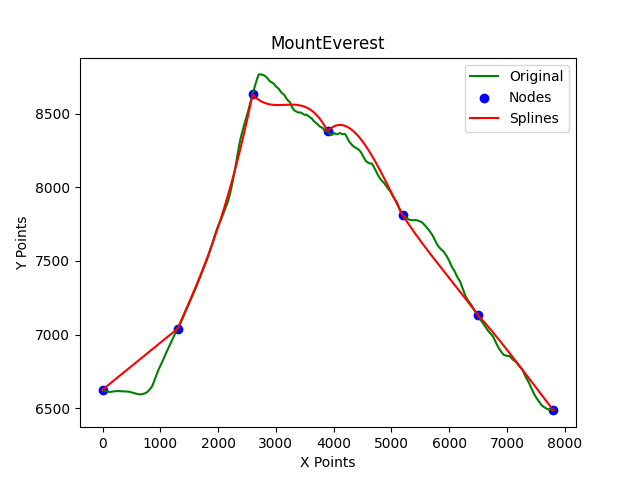
\includegraphics[width=\textwidth]{plots/MountEverest_splines_7.png}
        \caption{7 węzłów}
        \label{fig:7nodes}
    \end{minipage}
    \hfill
    \begin{minipage}[b]{0.49\textwidth}
        \centering
        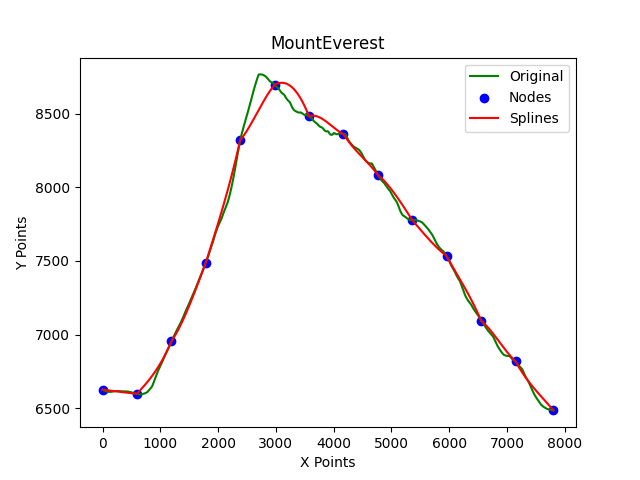
\includegraphics[width=\textwidth]{plots/MountEverest_splines_14.png}
        \caption{14 węzłów}
        \label{fig:14nodes}
    \end{minipage}
\end{figure}
\begin{figure}[H]
    \centering
    \begin{minipage}[b]{0.49\textwidth}
        \centering
        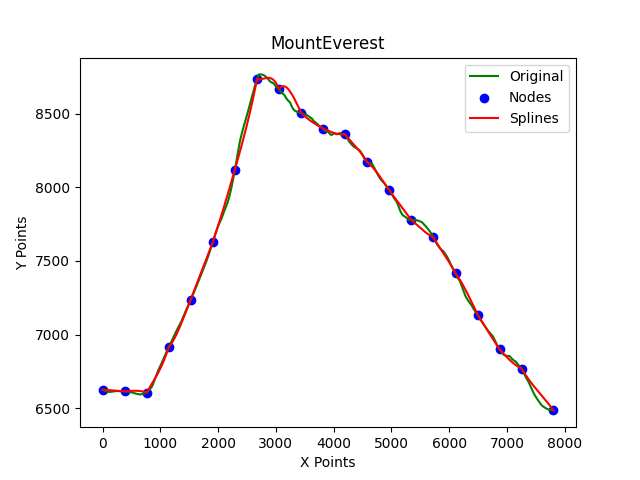
\includegraphics[width=\textwidth]{plots/MountEverest_splines_21.png}
        \caption{21 węzłów}
        \label{fig:21nodes}
    \end{minipage}
    \hfill
    \begin{minipage}[b]{0.49\textwidth}
        \centering
        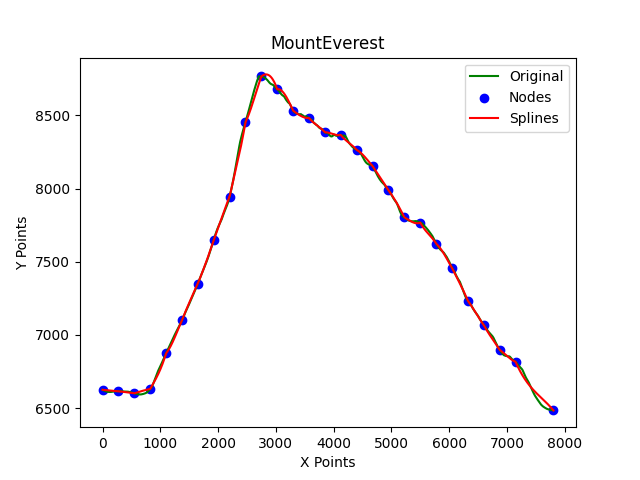
\includegraphics[width=\textwidth]{plots/MountEverest_splines_28.png}
        \caption{28 węzłów}
        \label{fig:28nodes}
    \end{minipage}
\end{figure}

Ponownie dzięki tej metodzie jesteśmy w stanie uzyskać znacznie lepszy efekt, szczególnie porównując wykresy do tych z metody Lagrange'a. Tutaj już przy 21 węzłach jesteśmy zaobserwować bardzo dobrą dokładność.

\clearpage
\section{Analiza dodatkowa}

Analiza dodatkowa polegać będzie na sprawdzeniu jak zachowuje się interpolacja dla różnych rodzajów terenu, jednocześnie zaimplementujemy węzły Czebyszewysza, aby sprawdzić jak zachowuje się funckja dla nierównomiernie rozłożonych węzłów. 

\subsection{Wielki Kanion Kolorado}

\begin{figure}[H]
    \centering
    \begin{minipage}[b]{0.49\textwidth}
        \centering
        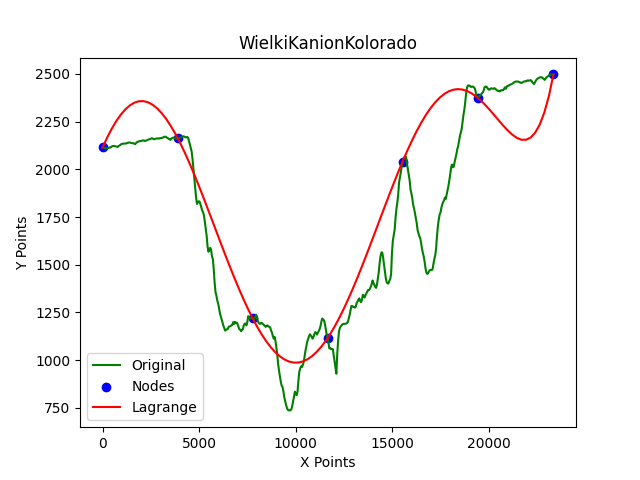
\includegraphics[width=\textwidth]{plots/WielkiKanionKolorado_lagrange_7.png}
        \caption{7 węzłów}
        \label{fig:7nodes}
    \end{minipage}
    \hfill
    \begin{minipage}[b]{0.49\textwidth}
        \centering
        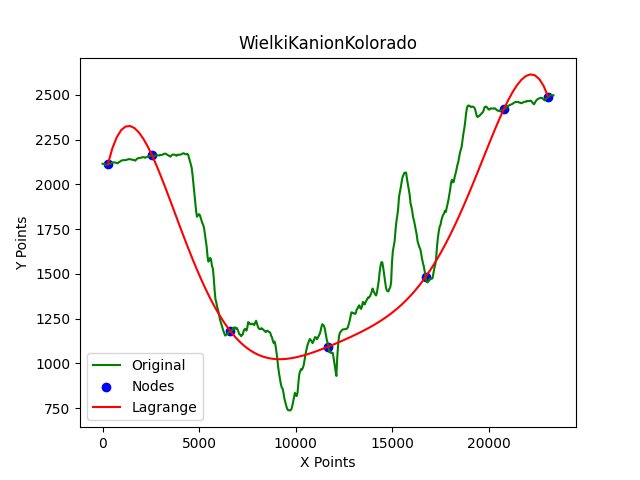
\includegraphics[width=\textwidth]{plots/WielkiKanionKolorado_lagrange_7_True.png}
        \caption{7 węzłów Czebyszewa}
        \label{fig:7nodes}
    \end{minipage}
\end{figure}
\begin{figure}[H]
    \centering
    \begin{minipage}[b]{0.49\textwidth}
        \centering
        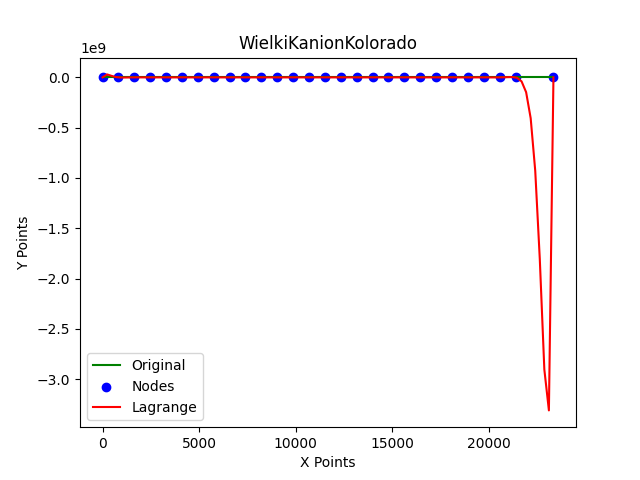
\includegraphics[width=\textwidth]{plots/WielkiKanionKolorado_lagrange_28.png}
        \caption{28 węzłów}
        \label{fig:7nodes}
    \end{minipage}
    \hfill
    \begin{minipage}[b]{0.49\textwidth}
        \centering
        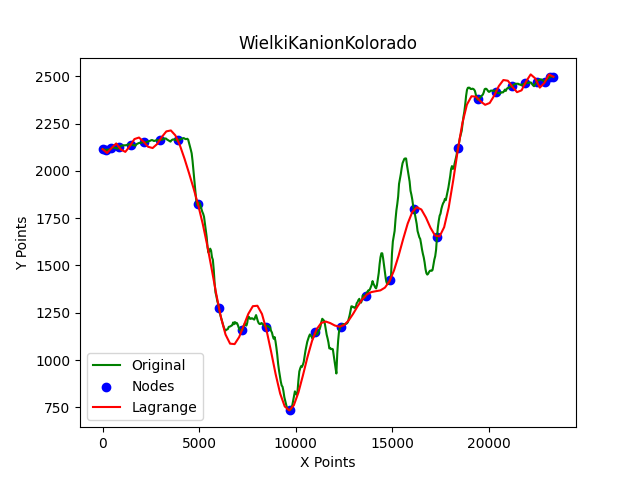
\includegraphics[width=\textwidth]{plots/WielkiKanionKolorado_lagrange_28_True.png}
        \caption{28 węzłów Czebyszewa}
        \label{fig:7nodes}
    \end{minipage}
\end{figure}

Na przedstawionych wykresach widać duża różnicę pomiędzy interpolacją Lagrange'a z użyciem węzłów Czebyszewa oraz bez ich użycia. Bez węzłów Czebyszewa funkcja jest wypaczona. Co prawda ich użycia dla tak zróżnicowanej trasy i tak nie daje nam bardzo dobrej dokładności nawet dla 28 węzłów.

\subsection{Stałe wzniesienie}

\begin{figure}[H]
    \centering
    \begin{minipage}[b]{0.49\textwidth}
        \centering
        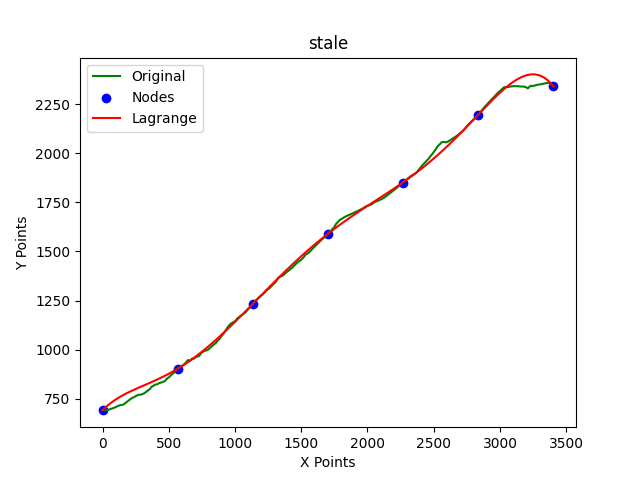
\includegraphics[width=\textwidth]{plots/stale_lagrange_7_False.png}
        \caption{7 węzłów}
        \label{fig:7nodes}
    \end{minipage}
    \hfill
    \begin{minipage}[b]{0.49\textwidth}
        \centering
        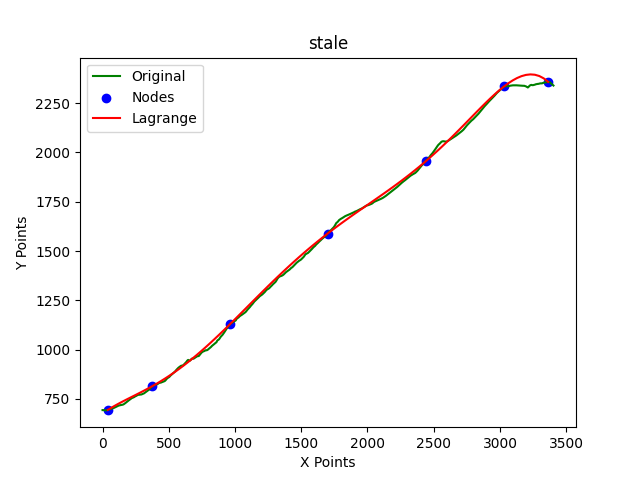
\includegraphics[width=\textwidth]{plots/stale_lagrange_7_True.png}
        \caption{7 węzłów Czebyszewa}
        \label{fig:7nodes}
    \end{minipage}
\end{figure}
\begin{figure}[H]
    \centering
    \begin{minipage}[b]{0.49\textwidth}
        \centering
        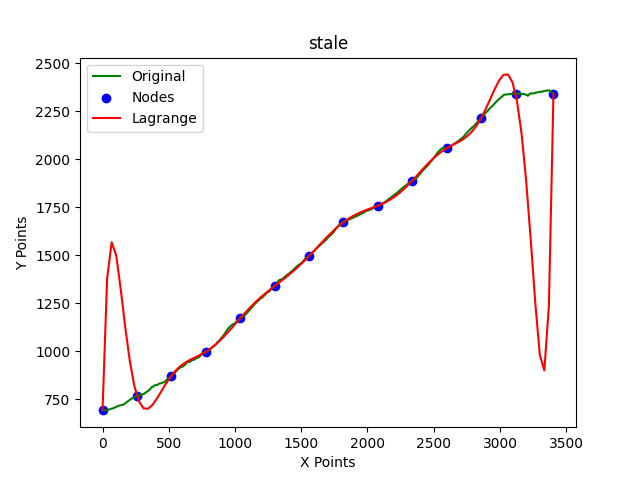
\includegraphics[width=\textwidth]{plots/stale_lagrange_14_False.png}
        \caption{14 węzłów}
        \label{fig:7nodes}
    \end{minipage}
    \hfill
    \begin{minipage}[b]{0.49\textwidth}
        \centering
        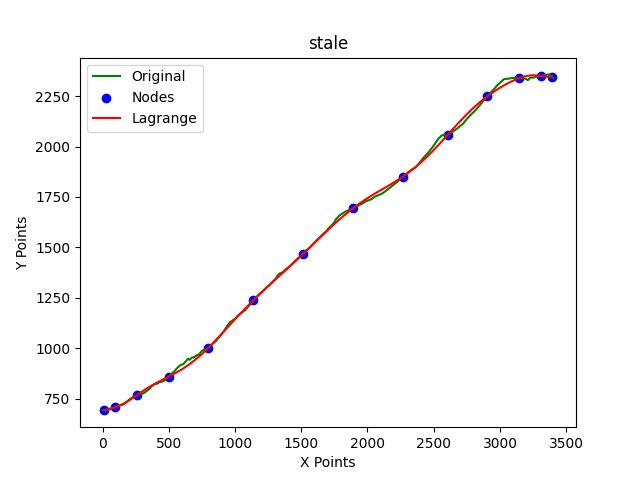
\includegraphics[width=\textwidth]{plots/stale_lagrange_14_True.png}
        \caption{14 węzłów Czebyszewa}
        \label{fig:7nodes}
    \end{minipage}
\end{figure}


Dla stałego wzniesienia widać dobrą dokładność już przy 7 węzłach, jednak kiedy nie używamy rożnorodnego rozstawienia węzłów, efekt Rungego wypacza wykres już przy 14 węzłąch, zapobiegają temu jednak węzły Czebyszewa.

\clearpage
\section{Podsumowanie}

W projekcie przeanalizowano dwie metody interpolacji: wielomian interpolacyjny Lagrange'a oraz funkcje sklejane trzeciego stopnia, stosując je do modelowania różnych profili wysokościowych. Metoda Lagrange'a, mimo swojej prostoty, okazała się podatna na efekt Rungego, który powoduje znaczące wypaczenia przy większej liczbie węzłów, zwłaszcza dla złożonych profilów terenowych. Zastosowanie węzłów Czebyszewa znacznie poprawiło dokładność tej metody, ale nie wyeliminowało całkowicie problemów dla bardzo zróżnicowanych tras. Z kolei funkcje sklejane trzeciego stopnia wykazały większą stabilność i dokładność. Tworzenie lokalnych wielomianów pozwalało lepiej dopasować interpolację do zmieniającego się terenu i unikać efektu Rungego. Dla większości analizowanych danych, dobre wyniki uzyskano już przy 21 węzłach. Stosowanie węzłów Czebyszewa w metodzie Lagrange'a znacząco poprawiło jakość interpolacji, szczególnie przy złożonych danych, poprzez zredukowanie błędów interpolacyjnych. Wnioski z analizy są następujące: metoda Lagrange'a, choć prosta, ma ograniczoną skuteczność przy dużej liczbie węzłów z powodu efektu Rungego, a węzły Czebyszewa poprawiają jej wyniki, lecz nie są idealne dla bardzo zróżnicowanych danych; natomiast funkcje sklejane są bardziej stabilne i dokładne, szczególnie przy większej liczbie węzłów, i lepiej radzą sobie z różnorodnymi profilami terenowymi.

\end{document}